% $Id: hardware.tex,v 1.8 2008/05/26 12:02:50 mrudolph Exp $

\section{\label{sec:stohard}Storage Manager Hardware}  %Editor: Gerry

\subsection{Overview of Baseline System} 
An overview of the existing  Storage Manager (SM) hardware configuration 
is given in Figure~\ref{fig:system}. 
The HLT nodes are grouped in subfarms and connected to two (soon eight) 
gigabit ethernet switches (Force10). 
Data from the HLT is sent to 8 SM nodes (Loggers). 
%The input bandwidth is provided by 6 GigE links per Logger node providing. 
%Currently only 2 switches are connected with 2 GigE links to each Logger node.
% resulting in a total bandwitdh of 2GB/s. 
The Logger nodes are also connected to a GigE switch (Tier0) to provide connectivity 
to the Tier0 system at CERN.
The connection to the NexSan SATABeasts is provided through two Fibre Channel QLogic SanBox 5600 
switches. Each NexSan SATABeast unit has two controllers with two fiber connections each. 
If one controller fails, traffic can automatically be switched to the second controller. 
The total network connectivity from the Logger nodes to the storage units is 8 times 2~Gb, 
such that the system is limited by the performance of the SATABeast controller. 
According to specifications each NexSan SATABeast should be able to reach up to $\sim$400MB/s write 
or $\sim$800MB/s read speeds, if equipped with a sufficient number of disks.
A system of 3 SATABeasts should be sufficient to meet a goal of 1 GB/s throughput,
and 6  SATABeasts the storage capacity goal.
However, the 8-fold symmetry of subfarms imposed by the connectivity 
of the 8 Force10 switches implies that efficient utilization of the subfarm resources
requires a multiple of 4 SATABeasts for balancing the load across the 8 subfarms.

% system overview
\begin{figure}[tbh]
\begin{center}  
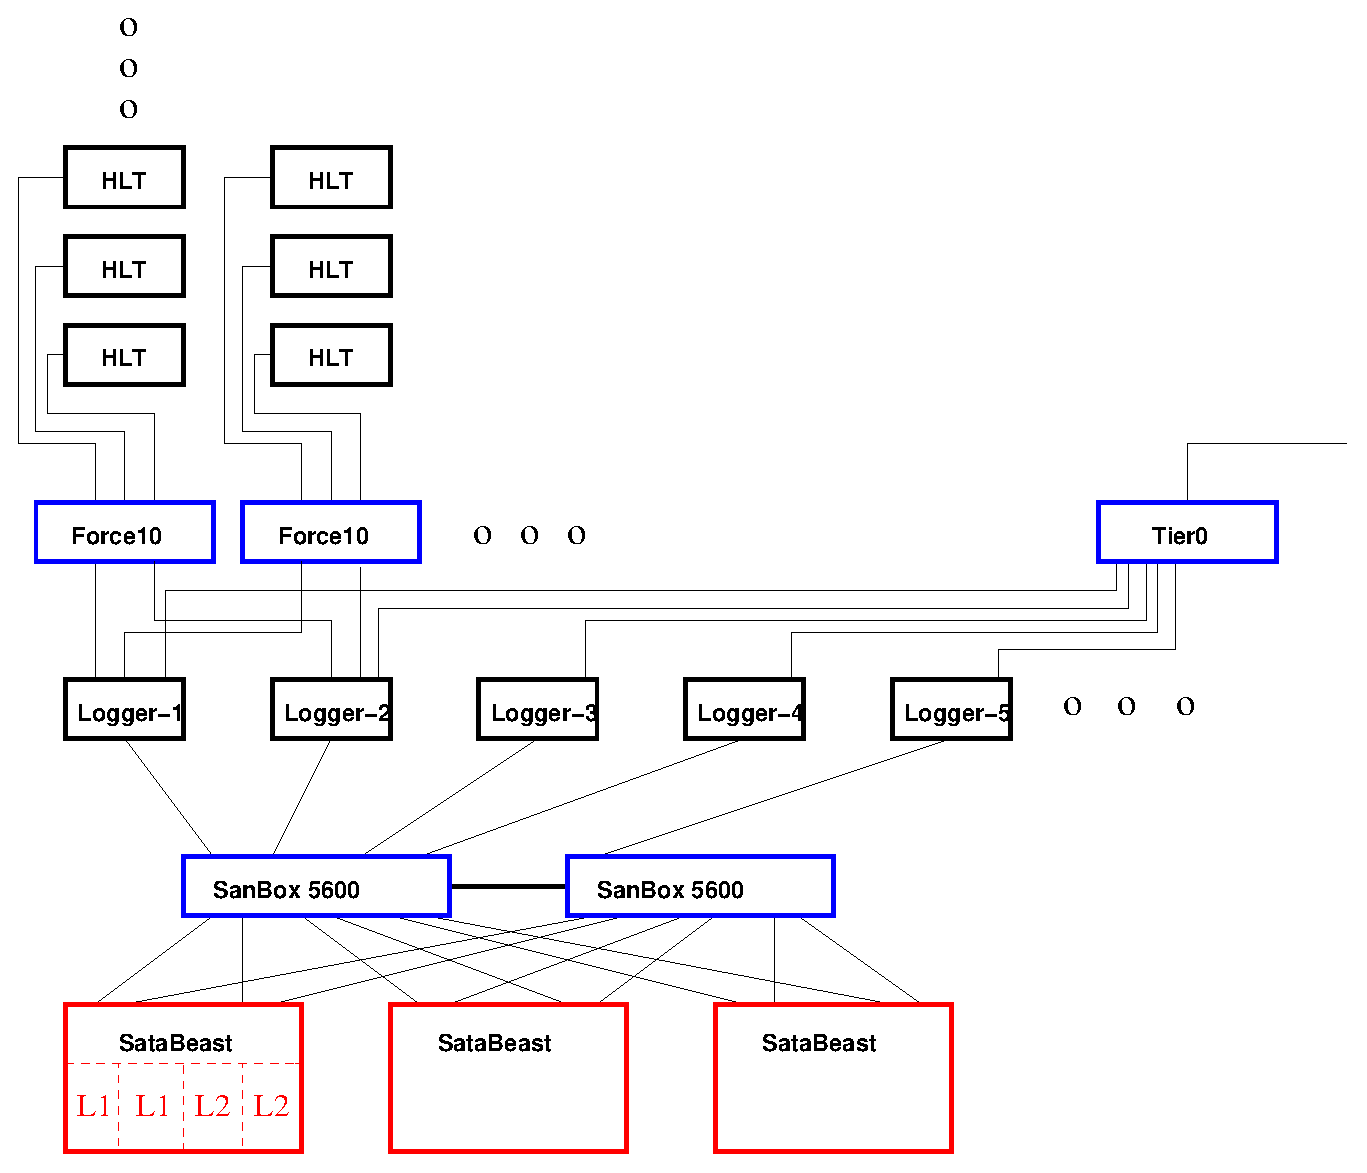
\includegraphics[width=1.0\textwidth]{Hardware/SMsystem}
\caption{\emph{ Storage Manager system overview of the currently installed hardware. 
The leftmost SATABeast is drawn indicating having the arrangement of four disk arrays, 
two arrays of which are ``owned'' by logger node 1 (``L1'') and two by logger node 2 (``L2'').}}
\label{fig:system}
\end{center}
\end{figure}  


\subsection{Hardware Components}

\subsubsection{Logger Nodes}
Logger nodes are standard Dell PC's PowerEdge 2950 with two dual-core Xeon processors and 4 GB RAM. 
Each node is equipped with a 4-port GbE card (Silicom PEG4i) and 
a fiber channel host bus adapter (QLogic QLE2460-CK). 
% An additional PCI-e slot is available for an extra 4-port GbE card if needed. 
The same PC's are used for the CMS HLT farm.
The SM nodes are fully incorporated in the DAQ group's Quattor system for managing 
the software installation of PCs.

\subsubsection{Fiber Channel switch}

The fiber channel switches are used to connect the logger nodes and the storage. 
Two QLogic SanBox 5600 switches are used. 
Each chassis includes sixteen 4Gb ports, plus a four-pack of high-speed 10Gb ISL ports 
of which one is used to connect the two switches.
The latter interconnect can be used to re-route traffic through the other switch
to reconfigure around the hardware failure of certain components.

\subsubsection{Storage Array}

The storage arrays are the SATABeast from NEXSAN. 
Each SATABeast has two controllers with two 2~Gb ports.
The total number of disk slots available is 42 and the system can support Sata disks 
of up to 1~TB size. 
NexSan SATABeasts have been successfully deployed for the CDF Consumer Server Logger system 
at Fermilab since 2006.

The arrangement and allocation of disks in the SATABeast is constrained by a number
of practical considerations.
Without substantial investment in a file management system it is simplest
to dedicate disk arrays to particular logger nodes, and given our use case, 
there is not much incentive to overcome this choice.
Due to its dual controllers, the SATABeast is best fed by two logger nodes,
implying a division of the SATABeast into an even number of disk arrays.
Given the  SATABeast capacity is for 42 disks, and the need for hot spares, 
the obvious choice is a configuration of four 10-disk arrays plus 2 hot spares.
By giving each logger node write control of two arrays, one can also obtain some benefit
from reading and writing from separate arrays, even though we do not plan
to enforce non-overlapping I/O. We can implement such a scheme if it is warranted.
The 10-disk arrays are also appropriate in that much smaller arrays would
suffer reduced throughput; and dramatically larger arrays would be at greater
risk for multi-disk failures, and longer re-build times.
The size of the disk arrays can be an issue for some file systems, 
but partitioning the arrays with multiple volumes easily avoids such limitations.

\subsubsection{Proxy Server Node}

As discused extensively in the software section, the SM supplies monitoring
data via a Proxy Server system.
Supplying and maintaining the hardware for the Proxy Server node 
is {\it not} part of the SM project, but a responsibility assumed by the DAQ group.


\subsubsection{Data Lookarea}

It is valuable for commissioning and data monitoring purposes to have rapid
{\it local} access to some fraction of the data recorded.
This has been addressed by copying the very first file of each run 
to a ``Lookarea'' which can be accessed locally at Cessy by users.
In the old small SM system of  \verb+cmsdisk1+ this was accomplished
by making a Lookarea directory on one of this machines data disks and
exporting to other nodes within the \verb+cms+ network.


For the SATABEast SM, however, we insist upon the policy that users
cannot have {\it any} externally driven interaction with the SM system.
Thus for the new SM a data disk is exported {\it to} the SM logger nodes,
the logger node initiates the copy of this first data file to this
external Lookarea machine, i.e. all interaction with the SM is under
SM control.
If the external node is unavailable, the file will not be copied, but
the SM will continue with its normal operation.

The PC serving the Lookarea disk is also a responsibility of the DAQ group.




\subsection{Storage Manager Performance}

The prototype system, currently installed in Cessy, has
3 SATABeasts installed  with 10 Sata disks of 750~GB  and 116 of 1~TB.
These are currently configured in our baseline in groups of 10-disk RAID5 arrays 
(2 spare RAID disks per SATABeast), yielding an effective capacity of 105.75~TB storage
for the full system.
With the dual controllers, a single SATABeast is expected to be fundamentally 
limited to about 400 MB/s writing.

The HLT subfarms are connected via a FORCE10 switch through
two 2~GbE Silicom links (``rails'') per logger node.
Presently the DAQ system is being recabled for the full contingent of eight FORCE10 switches
such that each switch, corresponding to a DAQ ``slice,'' has connectivity with 
a single SM logger node.
Another layer of a pair of additional switchs are being contemplated by the DAQ group
that would remove this restriction.
The Ethernet connection limits the theoretical wire-speed of data input
to a logger node to 250~MB/s.

Each logger node is connected to the Tier0 switch with a single 2~GbE link.  

The 3-SATABeast prototype system was designed to be able to provide a throughput of about 1~GB/s,
but it falls short of the design of 250~TB capacity. 
This requires an expansion of the system, which is discussed in Section~\ref{sec:SMexpansion}.
Because each SATABeast will collect the data from two DAQ slices, and the slice structure
is simple replication of parallel structures, a single SATABeast fed by two logger nodes
is the atomic unit for projecting throughput performance---although we usually quote
results on a per node basis, test numbers are
obtained using two nodes each accessing a seperate disk array unless otherwise stated.
We use this model in our performance studies and extrapolation to that of the full system.

The nominal setup for our system tests include the following features (unless stated
otherwise):
\begin{itemize}
  \item SLC4 Linux installation on logger nodes
  \item 2 logger nodes accessing separate ten-physical-disk arrays on the same SATABeast
  \item Each logger node has control of two arrays, and alternates the file writing
between these two arrays as luminosity sections are incremented
  \item 128k SATABeast stripe size (max allowed)
  \item RAID5 disk redundency
  \item XFS file system on the SATABeasts
  \item Single output stream
  \item $\sim$1 MB event size
  \item 1 GB data file size 
\end{itemize}
Our tests can be categorized in terms of subcomponent capability and full system tests.
Subcomponent tests include:
\begin{itemize}
  \item {\bf Ethernet Input on Logger Nodes:} The Ethernet throughputs have been tested for two cases.
First, we have set up the full DAQ readout chain but flagged all the data from FUs to the SM
to be a stream that is {\it not} written out. In this case a 1-rail SM sinks about 110 MB/s,
and a 2-rail SM takes in 220 MB/s.
Similarly, the single logger-node link to Tier0 for simple file transfers (with no other activity)
also saturates  at about  110 MB/s.
  \item {\bf Direct Logger Node Write/Rread to a SATABeast:} To gauge the write performance 
from a logger node to a SATABeast 3 GB files were generated by \verb+dd+ (64k block size)
and written to a  SATABeast disk array; read tests were done with 1 GB files. 
Early tests with few disks provided rather low rates, but
later we settled on 10-disk arrays as a compromise configuration. 
We obtained the following results:
%\begin{table}[h]
\begin{center}
\begin{tabular}{c|c|c|c}
\# nodes   & \# Arrays & Write Only (MB/s) & Read Only (MB/x) \\ \hline
1          &     1     &     198           &    211\\
1          &     2     &     198           &    200\\
2          &     2     &     377           &    383\\ \hline
\end{tabular}
\label{tab:ddrates}
\end{center}
%\end{table}
With two logger nodes we have driven the SATABeast near the expected 400 MB/s maximum.
Similar performance was seen with \verb+dc_bench+.

The choice of 10-disk arrays is, as much as anything, almost a forced choice
given that that the SATABeast is limited to 42 disks and at least 2 disk spares
seems to be a minimum choice, and one would like an even number of arrays.
However, in terms of \verb+dd+ write rates, 10 disks is also a good choice:
\begin{center}
\begin{tabular}{l|c|c|c|c|c} \hline
\# Disks:      &   6    &   7    & 8    & 10   &   13\\ \hline
Rate (MB/s):   & 160    & 174    & 180  & 198  &  200\\ \hline
\end{tabular}
\label{tab:ddrates2}
\end{center}
  \item {\bf Data Transfers to Tier0:} We have tested reading data files from
a  SATABeast via logger nodes and sending them out through a single  2~GbE link
to Tier0.
Dedicated read-only from the SATABeast, and using the standard \verb+CopyWorker+
transfer scripts, saturates the Ethernet at about 100 MB/s per logger node.
\end{itemize}

We can put all the pieces together in full system tests, 
which run the standard SM executables
and employ the full DAQ chain beginning from one or two crates of FRL's,  
run in a  mode where data was internally generated,
and have these event fragments built by the normal chain of RU's and BU's,
then feed to FU's, and finally
pass the events to the SM for recording over two Ethernet rails.
The filter algorithm of the FU has data  compression turned off and 
the event size was padded with dummy arrays to make it about 1 MB.

The operation of the SM consists of a series of stages which can be
functionally subdivided as:
\begin{enumerate}
  \item SM Receiving and handling events from the FU  
  \item SM Writing events to disk (each logger node alternates between writing to two of its own  arrays)
  \item For each file written: database operations for file bookkeeping and for the transfer system 
        are done by the SM executable
  \item Actual DB operations and transfer process of files to Tier0 are done by independent scripts
        (not by the SM executable) 

\end{enumerate}
The throughput rates measured for various permutations of these processes being
active or not in full DAQ running  are (in MB/s):
\begin{center}
\begin{tabular}{c|c|c|c|c|c} 
2. Write Files & 3. DB actions & 4. Transfer to T0 & SM Throughput  & Tier0 Rate& SATABeast Throughput  \\ \hline
   NO       &   NO       &    NO          &       220      &   --- &   ---       \\
 {\bf YES}  &   NO       &    NO          &       180      &   --- &   180       \\
 {\bf YES}  &  {\bf YES} &    NO          &       144      &   --- &   144       \\
 {\bf YES}  &   NO       &   {\bf YES}    &       150      &    50 &   150$+$50  \\
 {\bf YES}  &  {\bf YES} &   {\bf YES}    &       150      &    50 &   150$+$50  \\
\end{tabular}
\label{tab:rates}
\end{center}
These rates are quoted on  a {\bf per logger node} basis, although the measurements
were actually performed with two logger nodes feeding a single SATABeast.

It is interesting that there is a noticeable, and equal,  penalty for DB actions
and for transfers to Tier0, but one seems to ``shadow'' the other.
Also note that these test were done with the DB access managed by perl scripts invoked
by the SM executable. We have been in the process of restructuring this whereby
the DB access is entirely decoupled from the SM executable (see Section \ref{sec:fpt0}).
This may reduce the overhead delays in the SM from DB access.
We do not, however, count any performance improvement from this change.
This example highlights the fact that other fine-tuning of the system may be possible
and profitable for improving SM performance, but we note that this does not appear 
to be actually necessary for the SM to meet our original goals.

A further teasing apart of the effects on throughput is seen in an early
test with two SM nodes writing two arrays on a SATABeast, of 6 and 7 disks respectively,
that gave a rate of about 140 MB/s writing 1 GB files (no reads).
When each node was reconfigured to write the output in a {\it single} file of unlimited
size the rate increased to about  150 MB/s.

Questions about CPU load can only be fully addressed with all functionality
in place, including the eventual DQM load.
Howerver, a rough look at the \verb+top+ load when running the full DAQ chain and
transfers to Tier0 indicate the CPU is occupied $\sim$15-30\% by the system plus ``users,''
$\sim$20-50\% in I/O wait, and $\sim$20-80\% idle.
No problem is apparent at this point.
Heavier demands from additional tasks could change this picture, 
especially motivating an expansion of PC memory.

A variety of miscellanous issues were investigated with respect to throughput rates:
\begin{itemize}
  \item {\bf File Systems:}
Our initial choice for the file system was XFS.
However, during heavy loading with \verb+dd+ tests, and relatively rare incidents 
in full DAQ running,
we observed the logger nodes crashing (log messages indicated paging problems).
We tested a Linux kernel build under SLC5, and did not observe this problem.
However, operating with what is at this point non-standard software is not 
viewed as a very practical option.
We also configured the SATABeast file system under Ext3, and again did not observe
this problem.
In fact, most of the May Global Run (CRUZET-1) was run  with  Ext3
without any SM incidents.
We need to still be sensitive to possible negative impacts of choosing  Ext3 over XFS,
but so far we have not uncovered any major downside with running  Ext3,
and we have now adopted it as our default system.

  \item {\bf Multiple Output Streams:}
We have done a prelimiary test running the full DAQ chain to the SM with 
up to 5 output streams so far.
Interestingly the throughput performance showed a small increase 
in rate to 192 MB/s (compared to the benchmark of 180 MB/s).
When running with even more streams we ran into reliability problems
with the XFS file system (previous bullet).
These tests need to be extended with Ext3, but indications so far are
that multistreaming is not an issue.

 \item {\bf Large Number of Socket Connections:}
As a practical matter the SM is so far usually run with either a small number of FU's 
or  low throughput, and thus  one has  not been sensitive to the impact on performance 
of a SM node having to manage a large number of socket connections.
For 2008 LHC running the DAQ system expects to be running about 720 FU's---one
\verb+EventBroker+ (i.e. one socket connection to the SM) each.
With a 16-SATABeast system each logger node would support 45 FUs,
and any eventual system doubling would only push this 
to 90 FUs per logger.\footnote{Because of the finite rack space available, 
the DAQ group is significantly constrained that future increases of the filter farm take 
the form of larger numbers  CPU cores per FU rather than proliferating physical boxes.
This implies that even dramatic increases in CPU power of the filter farm
should not have a large effect on the connection load of the logger nodes.
Although, future upgrades with more rails is a possibility, but the capability
of the logger nodes would also presumably be improved.}
We ran a large connection test by feeding the output of 100 FUs into
a single SM (Ext3 file system, no DB actions, and no Tier0 transfers) and
achieved the usual write rate of 180 MB/sec.
An even larger system of 300 FUs showed only a modest drop to 150 MB/s.
\end{itemize}

Our essential conclusion is that while there may be worthwhile optimizations 
of the system, these results with one SM ``leg'' demonstrate that we are on track
to meet our performance goals even with the {\it existing}
state of the hardware and software.


\subsection{Hardware Expansion\label{sec:SMexpansion}}

The initial prototype system assembled in late 2007 was envisaged as Phase-I 
of a three phase expansion, the later phases were primarily to increase the
storage capacity.
Phase-II was to increase the disk inventory by 96 disks to fill up the existing
SATABeasts in the spring of 2008.
Phase-III was forseen for 2009 to essentially double the system for higher 
luminosity LHC running.
We have been operating under the general philsophy of this plan, 
but two developments have modified its execution.

First, we found that our testing of the system and providing support for CMS
running with a portion of the new SM hardware was, or would be, significantly hampered 
by the small inventory of disks on hand.
In particular, high data rates to the SATABeast is conditional upon have
fairly large disk arrays.
Therefore the Phase-II disk purchase was accelerated by a few months,
giving us in early April the 118.5TB currently installed.

Second, CMS management in consultation with DAQ and trigger
project managers concluded that the doubling the system in 2009 would be
better done  for the 2008 LHC run.
Essentially, in this early phase where operation may be unstable 
for the accelerator (e.g. store frequency)
and detector (e.g. triggering, zero-suppression,\ldots), 
it may be very important for CMS to be able to maximize  recording very high data rates
for the limited store-hours available.
The SM hardware team  was thus asked in May to quickly pursue doubling the system.
We have begun the process for purchasing the requested doubling, 
but have also incorporated two secondary design changes.

First, by virtue of the connectivity of the eight FORCE10 switches, the DAQ system
will have an explicit eight-fold symmetry in the data flow.
By having 8 logger nodes, the front end of the SM system is properly matched,
however, 8 nodes feeding 3 SATABeasts is not---the 8 nodes were originally 
conceived as 6 loggers $+$ 2 spares.
The SATABeasts are able to support eight slices,
but doing so breaks the natural topology of one node per  SATABeast controller.
This has the important impact that having 8 rather than 6 nodes will unbalance 
the throughput that the filter farms 
can support, and  the large investment in filter computing resources would be underutilized.
Thus the decision that the  SATABeasts should properly match the 8-fold symmetry
of the greater DAQ system, and that the prototype  configuration should consist
of four  SATABeasts rather than three.

A second modification of the design concerns the robustness of the system.
The Fiber Channel switches that move data from the logger nodes to the 
SATABeasts are fault tolerant, and allow traffic to be routed from one
switch to its partner and still make it to all SATABeasts. 
However, we have already experienced a failure of a switch {\it power supply}
and lost the connections for four of the logger nodes to the  SATABeasts.
To improve fault tolerance the expanded system will equip the logger nodes
with two Fiber Channel connections, one to each switch, so that complete failure of a switch
will not interrupt operation.

Aside from these two alterations, the system expansion is then a simple doubling,
and the final system for 2008 data taking should consist of:
\begin{itemize}
\item 16 logger nodes $+$ 2 hot spares
\item 4 Fiber Channel switches $+$ 1 pre-configured spare
\item 8 SATABeasts fully loaded with 42 disks
\end{itemize}
This system should readily exceed the original throughput/storage goals.

Assumming the purchase process and equipment delivery proceeds in a timely
fashion we would hope to have the full system in operation by the fall.


\subsection{SM Commissioning\label{sec:SMcommiss}}

The Phase-I system was installed in the latter part of 2007.
Performance studies were begun in Dec 2007 and carried out through the spring of 2008.
In Feburary 2008 the Tier0 connection was commissioned.
With the arrival of the supplementary disks (Phase-II) a SATABeast was configured
and ``delivered'' to the DAQ group in April for their routine use,
i.e. both for generic DAQ system tests and CMS data taking, especially for Global Runs.
This 1-SATABeast system includes two logger nodes, each assigned two 10-disk RAID5
arrays.

This 1-SATABeast system, in conjunction with the old MiniDaq SM which we continue
to support, has been more than adequate to serve CMS data taking needs.
We prefer to operate with the other two SATABeasts reserved for SM testing
and development, but on short notice, or for special purposes, we can devote
a second, or even the third SATABeast for CMS use.
Thus we are well positioned to support CMS needs.

In the short term future, conducting more realistic full-scale testing
is somewhat problematic from a variety of perspectives: 
the full DAQ system is not in place, 
and there is considerable demand for its resources purely from among DAQ developers;
a realistic data profile and final HLT algorithms are not in place;
and the DQM related impact upon the SM is not known as it is still under development.
We see meaningful large scale system tests of the SM will increasingly be integrated
within the context of overall large scale DAQ testing.
 

In fact, the proposal for the second  CRUZET global run in June are to run with a random trigger 
in addition to the cosmic trigger.
This will enable the DAQ system to be pushed to higher rates and heavier loads than
is possible with a high quality cosmic trigger. 
The unwanted random triggers can be identified in the  HLT filter for rejection.
We propose to divert these junk events a special stream, record them with the SM,
and even transfer them to Tier0, where they can finally be thrown away.
This will create a more challenging data load on the SM then in the past.
We envisage supporting four DAQ slices with four logger nodes and two SATABeasts.



Installation of the hardware for the SM expansion (Sec.~\ref{sec:SMexpansion}), 
assuming a rapid procurement process, should take place by the fall.
The physical installation of the new hardware is essentially a duplicate
system in a neighboring rack, and the assembly and commissioning work
would nominally be done with no interference of the existing system.
The exception is the 4th SATABeast to be installed in the old rack,
and installation of a second Fiber Channel port on the existing PCs.
This may in fact require some reorganziation of the existing rack, 
or at least presents a good opportunity to do so.
Ideally we would commission the new rack before embarking on any major
disruption of the old SM rack, but in any event, we would seek to maintain
at least one data-ready SATABeast at all times.
Our goal would be to have the entire expanded SM system operational
in early September.
% Operations Plans


\subsection{\label{sec:SMexperience} Storage Manager Operational Experience}

Throughout 2007 we supported CMS development, commissioning, and data taking
with the small provisional SM systems (\verb+cmsdisk0+ and \verb+cmsdisk1+).
This has continued in 2008, however,
since March a dual-node$+$SATABeast system has been dedicated
as the mainstay of CMS data taking.
We prefer to reserve the other two SATABeasts for technical development
and testing, but as the need arises we can quickly integrate one, or both,
of the other SATABeasts into normal CMS operations---it is largely an
administrative decision.

As an example of the use of the SATABeast by CMS,
the data throughput for the ``CRUZET'' Global Run is shown in Fig.~\ref{fig:cruzet}
for the two logger nodes.
Not surprisingly, cosmic ray running does not push the system very hard.
Operationally, once things are in place the Global Runs for the SM have
generally been smooth.
The run usually begins with a new, or even changing, software release,
and this means some setup issues are not always correct.
Once these are worked out, the SM running has been smooth except for one incident.
We began CRUZET using XFS (nodes 19 \& 20), and this seemed to caused a number
of incidents of node crashes.
Once we switched to Ext3 (nodes 15 \& 16), which is most of the data, 
no further SM problems were reported.

% cruzet
\begin{figure}[t]
\begin{center}  
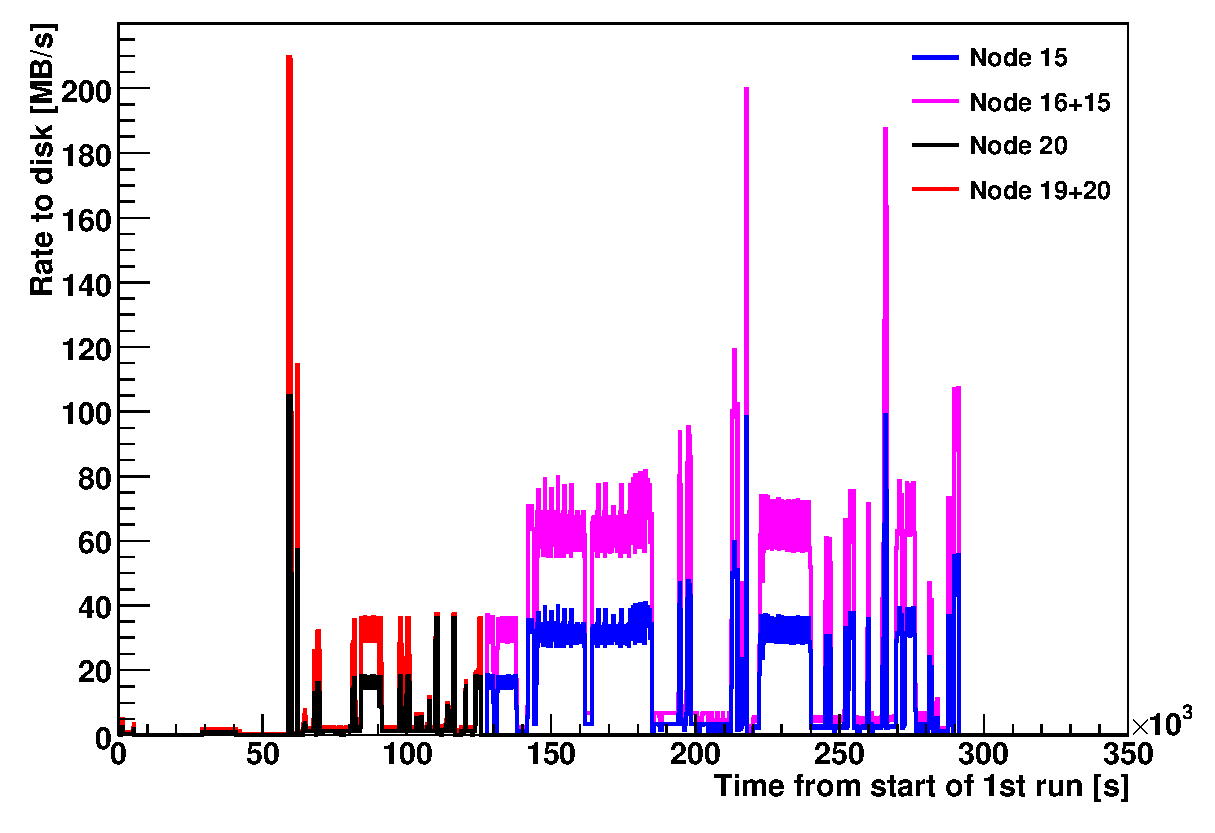
\includegraphics[width=0.9\textwidth]{Hardware/cruzetByNode}
\caption{\emph{Storage Manager throughput during the May 2008 ``CRUZET'' Global Run. 
The SM in CRUZET consisted of two logger nodes each running two SM instances,
thus making up a 4-Slice DAQ configuration; and the two logger nodes wrote
to a single SATABeast with 4 ten-disk arrays.
 The Global Run began with Nodes 19 and 20
writing to a single SATABeast with 4 disk arrays with the XFS file system.
Later in the run we switched to Nodes 15 and 16 writing to a SATABeast withh the Ext3
file system.
The lower traces are the throughput of one of the two nodes
(either 15 or 20), and the upper trace is the the total through put for
the two nodes (either 15$+$16, or 19$+$21). 
The SM used only a single ``rail'' each, and thus the spikes are reaching the network 
maximum of about 220 MB/sec total throughput. The spikes are brief occurances
due to trigger tests or improper trigger settings, 
i.e.  trigger rates for meaningful cosmics do not drive such high data rates.}}
\label{fig:cruzet}
\end{center}
\end{figure}  

For operation of the expanded SM system, we
would hope that timely processing and delivery of the new
hardware (Sec.~\ref{sec:SMexpansion}) would allow the full system 
to be in operation in September. 


\subsection{Response Plans for Hardware Failures \label{sec:SMhardfail}}

In order to minimize or avoid system down-time we envisage the following
sorts of protection against hardware failures.

\begin{itemize} 
\item {\bf Logger Node Failure:} We plan to pre-configure 2 PCs as ``warm'' spares.
The PCs would be equiped and tested with the full networking capability.
Due to the lack of spare ports for the switches, and the fact that
a preconnected spare that is truly ``hot'' will have a new identity
that would require a new DAQ configuration to be made (an expert activity),
it is deemed preferable to have ``warm'' spares which have been tested
to have full functionality, but to have them assume the host name of the
failed logger node via a Quattor system installation.
Since all DAQ PC's are administered via the Quattor management system
it is quick and easy (but still an expert action) to install a new PC with
the identity of a defunct node.
Then in addition to moving a few cables the spare node would fully assume
the old identity and be completely
functional in the existing DAQ system configuration. 

\item {\bf Fiber Channel Switch Failure:} The Fiber Channel switches have 
their own level of fall-over protection, in particular, traffic can
be rerouted to the partner switch.
However, catastrophic failures, like a complete power supply failure
can still bring down the switch.
Therefore our plan is to configure the expanded system with 2 fiber links
from each PC, one of which will be connected to each switch.
The SATABeast already has this dual connection split over the two switches.
This will then enable a complete and utter failure of a fiber channel
switch without impacting operations.
Furthermore, in the enlarged system with 4 switches in use, we plan to
pre-configure a hot spare switch which will only require moving optical
cables in order for it to take over from the failed unit.
Parenthetically, we note that this spare would also be of utility
in the event of a fiber channel switch failure in the CMS DB
installation at Cessy,  which has no spare in-hand.

\item {\bf SATABeast Controler Failure:} A part of the standard SATABeast 
design is the ability to be configured such that if one controller fails the second 
one can pickup the traffic without interruption.
We have not yet tested this feature, or seen the performance impact.
However, as each controller will only be supporting 1/16 of the data flow,
this should not have a dramatic impact.
We are investigating the particular procedures and response times
for Nexsan to provide replacement parts.

\item {\bf SATABeast Disk Failure:} The purpose, of course,
of the RAID array is that a disk may fail without loss of data.
Our baseline  mode of operation is to run RAID5 which will tolerate
a single disk failure.
Depending on the expectations of data demands, and experience with failures,
we may consider RAID6, allowing two disk failures in the same array.
With our division of four 10-disk arrays, and 2 hot spare disks,
and an assumed disk failure rate of 5\% per year, one in fact expects
to replace 2.1 disks per year per satabeast.
In a 3-day period (eg over a weekend) there is about 1.6\% average probability
of a single disk failure out of 40 disks---assuming uncorrelated Poisson statistics,
this drops to $1.3\times 10^{-4}$ for two or more disks failing in that 3 day window
(not necessarily in the same array).
RAID5 operation seems well warrented for these average statistics.
However, as disks age this average estimate may be too optimistic,
and a more mature system in later years may warrent revisiting these numbers.

A disk failure does not lose data, but could yet impact performance.
We exercised the RAID rebuild function of the SATABeast to understand the
impact on data rates.
Rebuild times are quite substantial, and depend on array size and the rebuild 
Priority setting. A small 4-disk array rebuilds in 8.4 hours for the highest
priority, and 11.1 hours in the lowest priority---all with no other activity on the SATABeast.
A 10-disk array takes 13.3 hours at the highest priority.
We started a run of the full DAQ chain to a single logger node 
to a single SATABeast array and were obtaining stable write speeds 
(no transfers or DB activity) 
of about 194 MB/sec (writing to a single array with XFS), 
and then triggered a simulated  disk failure {\it during} the run.
The write speed only decreased to 188 MB/s, but the rebuild rate dramatically increased.
Writing overlapped with the disk rebuild for about only 7 hours, after which
the  two arrays were actually filled up (there were no transfers for file removal),
but it nevertheless still almost took 22 hours to finish the rebuild.
We conclude that disk rebuilds have essentially no impact on performance,
but do take a very long time overwhich the array is still vulnerable.

\item {\bf Loss of Tier0:} The connection to, and operation of, the Tier0 center
is not our responsibility, but obviously is a potential impact.
The purpose of the large storage capacity planned for the SM was
aimed at this potential problem.
The size of the SM capcity was motivated to be able to sustain CMS data taking
through a weekend plus a day with the complete loss of Tier0 transfers.
We presume Tier0 services can be restored within this time frame.
\end{itemize}

With the exception of the loss of a logger node, none of these failures
require immediate response on the part of the shift crew.
The most expediant response to the loss of a logger node is
to reconfigure the DAQ to either drop the slice, 
or redstribute the traffic from the FU's.
This problem scenario is not very much different from the loss of a RU
at the beginning of the chain.
Thus reconfiguring the DAQ is a broader issue for the DAQ group.


In practice, most problems encountered are not these catastrophic hardware failures,
but smaller annoying problems arise for the shift crew like stopping executives on 
encountering of a configuration failure or general run-time failures,
We currently have been handling these problems by being experts-on-call.
In the future data-taking periods, the DAQ group will take more integrated
approach to having a generic on-call person with semi-expert knowledge to take 
care of a broad spectrum of remedial fixes.
Only after that line of defense has been exhausted would experts be called.
We have begun some documentation along these lines, but important
aspects of the system have been in flux and we most of this task
remains to be done.


\subsection{Personnel Support for Hardware Commissioning and Operations}

At the time of the last review, in Nov 2007, the MIT hardware team 
was undergoing major personnel changes.
This centered around the then immenent departure of Markus Klute
to a faculty position, and the review committee expressed
some concerns as to the adequacy of human resources.


In late November, Research Scientist Gerry Bauer joined the SM project
full time, and thesis student Matt Rudolph joined part-time while still maintaining
activities in the tracker group.
A search was begun for a relacement of Klute, and this gap was
filled in March 2008 with the addition of Constantin Loizides,
a physicist with IT training, to the  MIT SM team. 
In early June the MIT team will be further enhanced by the addition
of Josep Serrano, an IT professional, as System Administrator.
Christoph Paus continues his leadership, now as a formal USCMS 
L-3 project co-manger along with Harry Cheung.

In summary, MIT maintained continuous personnel support of the SM hardware project 
through the departure of M. Klute, and further expanded the level of support
commensurate with the enlarged system.
We are confident that we have the necessary personnel to meet SM commitments,
and that the initial cautions expressed by the reviewers 
has been well addressed.


\subsection{Hardware Cost and Future Projections}
Table~\ref{tab:proto} shows the costs for the proto-type system purchased in 2007 
with the exception of the Logger nodes, Silicom cards and fibers, 
which where ordered together with the nodes used for the HLT farm or a database project,
and supplied by CERN. 
In total \$80k were spend on the proto-type system. 

A cost summary for hardware through 2010 is summarized in  Table~\ref{tab:costs}.
It includes the expenditures for 2008, which are either completed
or based on quotes supplied by vendors, except for an year old estimate 
for optical fibers.
The 2009 and 2010 projections costs are based on current costs,
with no attempt to account for falling technology prices or inflationary increases.

No new major purchases are forseen for 2009 or 2010, 
however, warrenty periods will be expiring, and in particular our original
three SataBeasts will go off warrenty in 2010.
Hardware failures are of course unpredictable, but we have separated
our estimates in terms of `disks' and 'Misc. Hardware' as  statistical
projections of disk failures are more meaningful with our large sample.
The funds listed under ``Misc. Hardware replacement'' would be sufficient
for one major sub-component failure (e.g. $\sim$\$5k for SataBeast controller) and
still leave a small reserve for other small component failures.
This division is of course only conceptual, and
actual experience will dictate the ultimate allocation of funds for replacement 
hardware.

\begin{table}[!ht]
\begin{center}
\begin{tabular}{l|r|r}
year & cost    & product \\\hline\hline
2007 & \$66k   & 3 SataBeasts with 10 disks  \\\hline
2007 & \$6k    & 2 QLogic switches$+$hardware  \\\hline
2007 & \$8k    & 8 QLogic HBAs \\\hline
2007 & \$4k    & 2 QLogic switches hardware \\\hline
2007 & CERN    & 8 Dell PowerEdge 2950 PCs\\\hline
2007 & CERN    & 8 Silicom PEG4i \\\hline
2007 & CERN    & 20 2m fiber \\\hline\hline
\end{tabular}
\caption{Prototype system costs.}
\label{tab:proto}
\end{center}
\end{table}

% Second Fibre Controller (2 fibre and 2 iscsi ports) Pricing $4,922
% FC switch: ~3k

\begin{table}[!ht]
\begin{center}
\begin{tabular}{l|r|r}
year  & cost      & product \\\hline\hline
2007  &     \$80k & prototype system \\ \hline\hline
2008~~Feb&  \$46k & 100 1TB  SATA disks  \\\hline
2008~~May& \$182k & 5 SataBeasts with 42 disks  \\
         &  \$11k & 25 Spare 1TB SataBeasts \\
         &  \$16k & 2QLogic switches$+$hardware  \\ 
         &  \$25k & 20 QLogic dual HBAs \\\hline
2008     &   \$1k & 50 2m-optical fiber \\\hline
2008     & CERN   & 10 Dell PowerEdge 2950 PCs \\\hline
\hline
2009     &  \$11k & 25 Replacement 1TB disks \\ \hline
\hline
2010     &  \$11k & 25 Replacement 1TB disks \\ \hline
2010     &   \$7k & Misc. Hardware replacement  \\  \hline
\end{tabular}
\caption{Storage Manager system costs to 2010.}
\label{tab:costs}
\end{center}
\end{table}

%% 
%% \begin{table}[!ht]
%% \begin{center}
%% \begin{tabular}{l|r|r}
%% year & cost    & product \\\hline\hline
%% 2007 & \$80k   & proto-type system \\\hline
%% 2008 & \$51k   & 96 SATA disks  \\\hline
%% 2009 & \$66k   & 3 SataBeasts with 10 disks  \\\hline
%% 2009 & \$51k   & 96 SATA disks  \\\hline
%% 2010 & \$17k   & Hardware replacement  \\
%% 
%% \end{tabular}
%% \caption{OLD:: Storage Manager system costs.}
%% \label{tab:costsOLD}
%% \end{center}
%% \end{table}
%% 
%% 

% memory expansion??

%% operations: 24/7 coverage plans

%% system monitoring -- faults, perform feedback, tuning...shift crew feedback

%% no requirements doc, defining divisions & boundaries ??==> sm proposal doc

%% accept amount of data can be lost?

%% disk layout on sata--a baseline

%% disaster recov?

%% interaction & misbehavior of other systems?

%% doc & proc in place before startup

%% self repairable system...

%% means of quick re-config

%% costs: add service contract --- sata replacement after 5 yr  <-- too far out 

%% Qlogic warrenty on HBA 3 yr, switches 2 yr

%% disk frag impact on writing --- very file sys dependent --- killed sys in past
